\documentclass[a4paper, 10pt]{article}
\usepackage[utf8x]{inputenc}
\usepackage{graphicx}
\usepackage{geometry}
\usepackage{amsmath}
\usepackage{mathenv}
\usepackage{amssymb}
\usepackage{amsfonts}
\usepackage{mathrsfs}
\usepackage{textcomp}
\geometry{hmargin = 2.5cm, vmargin = 1.5cm}

%opening
\title{GE20 - Dropbox}
\author{Pierre-François Rouleau - Antoine Hars}

\begin{document}

\maketitle

\section*{Introduction}
Dans le cadre de l'uv GE20 (Économie Industrielle),
nous avons réalisé une étude de cas d'une entreprise ou d'un secteur de marché.
Nous avons donc choisi de nous intéresser au cas de l'entreprise DropBox,
qui en l'espace de quelques années, est devenue une référence dans le domaine du stockage en ligne de fichiers.\\ \\

\section*{1. Exposition du cas}

\subsection*{a) Le contexte.}
De nos jours, la consommation de services ne cesse d'augmenter, en plus de la consommation de produits issus de l'industrie.
Cette consommation croissante de services, soutenue par une évolution constante des technologies informatiques, permet aux consommateurs
de changer leurs habitudes comme par exemple dans le domaine du stockage de données.\\ \\
Nous pouvons prendre comme exemple les évolutions des habitudes des consommateurs pour le transfert et le transport de fichiers :
D'une utilisation de supports physiques de type clé usb ou disque dur portable, les utilisateurs ont tendance à se tourner vers des solutions
ne requérant aucun support physique comme le stockage en ligne sur des serveurs distants.\\
On utilise le terme de \textit{Cloud Computing} pour désigner les techniques de sauvegarde distante de données sur des serveurs.
En utilisant cette façon de faire, les utilisateurs du \textit{Cloud} n'ont pas à se soucier du support pour la sauvegarde mais
seulement des donn\'ees sauvegardées.\\ \\
Cette évolution dans le stockage apporte une plus grande simplicité pour les utilisateurs
qui n'ont besoin que d'un ordinateur et d'une connexion internet pour recueillir leurs données
au lieu de devoir faire\\attention aux différentes clés usb que les consommateurs peuvent avoir.\\
Il y a un phénomène de Destruction Créatrice (énoncé par Schumpeter), de transfert de compétences entre ces deux domaines.
La nature des biens consommés et utilisés par les consommateurs change.\\ \\
Nous avons pu observer qu'un de ces services de \textit{Cloud Computing} connaissait un plus large succès
que ses concurrents auprès des consommateurs : Le service DropBox.\\
Nous avons donc choisi de nous intéresser et d'étudier ce service tout particulièrement.\\ \\
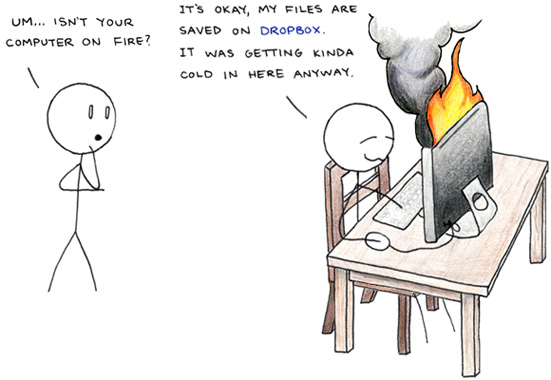
\includegraphics[height = 6cm, width = 6cm]{jpg/db1.jpg}
\newpage

\subsection*{b) Présentation de DropBox.}
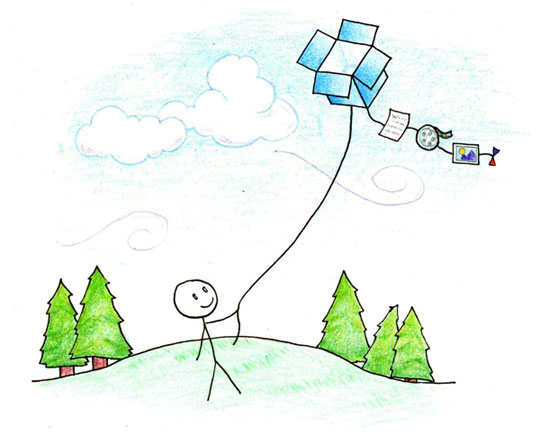
\includegraphics[height = 5cm, width = 5cm]{jpg/db2.jpg}

\includegraphics[height = 2cm, width = 6cm]{jpg/dropbox_logo.png}\\
DropBox est un service de stockage et de partage de fichiers en ligne permettant à ses utilisateurs de stocker et
de synchroniser des fichiers entre plusieurs ordinateurs.\\
Ce service s'est fait surtout connaitre du grand public par son refus de rachat
par l'entreprise Apple pour un montant de 800 millions de Dollars.\\ \\
Ce service se veut simple d'utilisation et ce sur n'importe quelle plateforme.
Il fonctionne donc sur les systèmes d'exploitation Windows, Linux et Mac, ainsi que sur les appareils de type Smartphone et Tablette).\\ \\
L'origine de ce service vient de l'envie, de la part de ses créateurs Drew Houston et Arash Ferdowsi (deux anciens étudiants de la MIT),
de palier aux soucis liés à l'utilisation de supports physiques tels que la perte, l'oubli et la destruction d'une clé usb par exemple.\\
Les deux fondateurs du service DropBox ont donc choisi de fonder leur startup en 2007.\\
Ils ont ensuite lancé le déploiement de leur solution de stockage en ligne courant 2008.\\
L'entreprise est localisée à San Francisco en Californie.\\ \\
DropBox est un service principalement centré sur le B2C (Business to Customer) mais commençant à s'intéresser au B2B (Business to Business),
s'adressant donc autant aux entreprises qu'aux particuliers.\\ \\
Au niveau de ses acquisitions depuis sa création, DropBox en a effectué plusieurs comme :
\begin{itemize}
 \item Le rachat de \textbf{Cove}, un outil puissant de collaboration dans l'élaboration de projets informatiques.
 \item Le rachat du service \textbf{AudioGalaxy} qui proposait un outil de partage de musiques.
 \item Le rachat de l'entreprise \textbf{Snapjoy} pour une meilleure intégration des photos dans DropBox.
 \item Le rachat de la startup \textbf{TapEngage} pour une gestion et un affichage efficaces des publications et des annonces
sur différentes tailles d'écran.
 \item Le rachat du client de messagerie \textbf{MailBox} de la compagnie Orchestra pour un montant de\\100 millions de Dollars
afin de permettre de stocker des données dans son Cloud tout en les rendant accessibles depuis son service de messagerie
(Google a le même fonctionnement avec Gmail et Drive, un service similaire à DropBox).
\end{itemize}
Ces acquisitions nous ont permis d'observer que DropBox tend à être plus qu'un simple système de stockage de données en ligne,
mais souhaite proposer à ses clients, une solution, un service capable de gérer de manière simple et efficace
tous les types de fichiers courants.
Par exemple, pouvoir écouter sa musique sans avoir le fichier d'une chanson sur son appareil,
pouvoir partager et surtout regarder ses photos facilement.
DropBox souhaite aussi offrir une solution générique permettant de gérer ses données stockées sur le Cloud en y associant des mails.\\ \\
En 2012, DropBox a effectué une levée de fonds valorisant la société à un montant de 4 milliards de dollars et
prépare son entrée en bourse pour le deuxième semestre de l'année 2013.
\newpage

\subsection*{c) Le fonctionnement du service DropBox.}

\includegraphics[height = 4cm, width = 4cm]{jpg/dropbox_1.png}
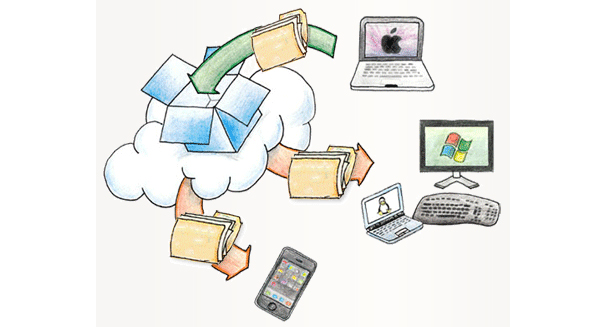
\includegraphics[height = 3cm, width = 6cm]{jpg/dropbox_3.jpg}\\ \\
Pour permettre d'avoir accès à ses fichiers sans support physique de type usb, DropBox fonctionne de la manière suivante :\\
Lors de l'installation de l'application sur la machine d'un client, un agent est installé.\\
Cette agent a pour but d'envoyer chaque modification de fichier observée sur les serveurs de l'entreprise DropBox.\\
Une fois le fichier enregistré sur un des serveurs de DropBox, il est transféré sur toutes les machines abonnées
au compte du client effectuant la manipulation.\\
Les agents de synchronisation de chacune des machines se chargent donc de recevoir des serveurs les modifications de fichiers pour
finaliser la synchronisation des fichiers entre les différentes machines à\\disposition du client.
Nous pouvons dire que tout changement dans un dossier DropBox donne lieu à un évènement qui, si le fichier est modifié,
déclenche une synchronisation du dît fichier.\\ \\
Un point important de l'utilisation d'un service de type DropBox vient du fait que les données sont hébergées localement d'une part
et sur un serveur distant d'autre part (nous pouvons utiliser le terme de cloud ou nuage pour définir cette sauvegarde
sur un serveur distant).
Cette sauvegarde à distance apporte un mécanisme d'historisation des modifications et 
permet donc aux utilisateurs de rattraper les éventuelles erreurs opérées sur leurs fichiers et
surtout les suppressions non-voulues de fichiers.\\ \\
Grâce à ce service, il n'est plus question de se soucier de l'utilisation d'un support physique pour\\transporter ses données
ou de l'utilisation des envois de fichiers par email pour récupérer ses données.\\
Et concernant la sécurité dans le stockage des données, les communications pour la synchronisation des fichiers sont cryptées et
les dossiers privés le sont eux aussi. Ils ne sont accessibles que par les personnes que le client a invité.\\ \\

\subsection*{d) Les statistiques de DropBox.}
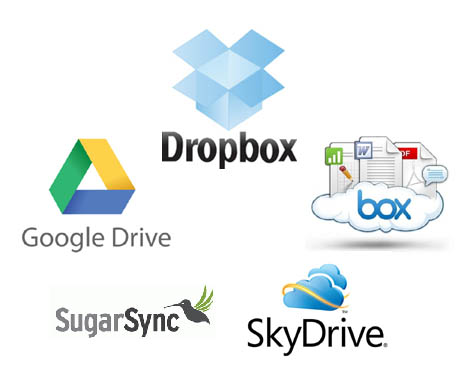
\includegraphics[height = 3.5cm, width = 3.5cm]{jpg/db4.jpg}\\
Dans un secteur où la compétition est rude avec beaucoup de concurrence
(on a dénombré une vingtaine d'applications de stockage en ligne dont Box, Skydrive de Microsoft, Google Drive, iCloud d'Apple,\\SugarSinc,
etc..), DropBox a su croître très rapidement :\\
Fin 2008, ce service comptabilisait un total de 100 000 utilisateurs différents.
En 2009, il en comptait\\2 millions, 4 millions en 2010, 25 millions en 2011 et
à la fin 2012, l'entreprise comptabilisait 200 millions de clients différents.\\
L'application est installée sur pas moins de 250 millions d'appareils et
en terme de fichier, 1 milliards de fichiers sont sauvegardés tous les 48 heures.\\ \\
Du point de vue financier, DropBox comptabilise une centaine d'employés et générait des revenus à hauteur
de 240 millions de Dollars en 2011.\\
Nous pouvons dire que le service DropBox ne déroge pas à la règle de l'effet réseau énonçant que l'utilité d'un service
a tendance à augmenter avec le nombre d'utilisateurs, ce qui a pour conséquence de créer une cristallisation autour de cet acteur
par rapport aux autres.

\newpage
\subsection*{e) L'économie associée à ce service.}
Le service Dropbox est découpé en 2 sections pour appliquer le modèle économique Freemium:
\begin{itemize}
 \item Une offre gratuite de base.
 \item Une offre premium payante.\\
\end{itemize}
Les clients se voient offrir un compte gratuit lors de l'inscription avec un espace de stockage limité à\\2 Go.
Pour bénéficier de plus d'espace de stockage, les clients ont plusieurs possibilités.\\
Ils peuvent :
\begin{itemize}
 \item Parrainer de futurs clients en fournissant un lien spécial d'inscription.
À chaque fois qu'un nouvel utilisateur s'inscrit en utilisant ce lien, 500 Mo sont ajoutés au compte parrain.
Au final, il est possible de parrainer un maximum de 32 amis pour obtenir de l'espace de stockage ce qui correspond à 16 Go.
 \item Se connecter aux réseaux sociaux (Facebook et Twitter).
 \item Donner son avis sur le service DropBox.
 \item Exécuter toutes les étapes de prise en main du service DropBox.
 \item Basculer son compte gratuit en compte premium payant qui nous permet d'ajouter un espace de 100 Go, ou 200 Go ou encore 500 Go.
 \item Basculer son compte gratuit en compte entreprise qui se tourne vers les entreprises désirant intégrer le \textit{Cloud Computing}
dans leurs processus de production.\\
Dans ce cas de figure, la taille de l'espace de stockage n'est plus le point primordial de l'offre mais
plutôt le nombre de personnes qui interagissent en même temps sur le projet.\\
Le service DropBox pour ce cas, offre une plus forte sécurité,
un support téléphonique et les outils nécessaires pour la gestion des versions d'application.\\ \\
\end{itemize}

\subsection*{f) La réussite de DropBox.}
Du fait de sa simplicité d'utilisation, DropBox se démarque de ses concurrents et
a atteint 50 millions de clients actifs en seulement quelques années,
tout en sachant qu'environ 96\% de ces utilisateurs possèdent un compte classique (non payant).\\
L'impressionnante réussite de DropBox par rapport à ses concurrents vient du fait que dans un premier temps,
il s'agit d'un service simple et disponible sur toutes les plateformes du marché et
que dans un\\second temps, ce service dispose d'une communautée d'utilisateurs très présente et soucieuse
de\\contribuer à l'amélioration du produit.\\ \\
DropBox s'inscrit plus dans une thématique de proposition d'un service global que de services.\\
Ces concurrents sont plus dans une optique de prestations immatérielles avec peu de prises en compte du retour client.
Cela conduit au besoin d'une forte publicité pour recruter des clients
car ceux-ci expriment moins de recommendations que si leur avis comptait.\\
Et depuis la réussite du service DropBox, de plus en plus de services similaires s'inspirent de ses méthodes de pénétration de marché.\\ \\
Dans le cas de DropBox, le client est au coeur du produit où le but est de rendre service avant tout.\\
Ce produit propose une solution à un problème en restant le plus proche des besoins des clients.\\
DropBox a su imposer un service, non primordial pour les consommateurs en amont,
mais rapidement devenu comme indispensable pour ces clients, les risques étant de proposer un produit qui n'intéresserait personne.\\
Avant l'arrivée de DropBox sur le marché, des systèmes de stockage et de partage de fichiers en ligne avaient déjà été mis en place
mais aucun n'avait su s'imposer auprès du grand public car ne proposant pas un produit simple et utilisable sur tous les supports disponibles.
Ces systèmes étaient plutôt utilisés par des utilisateurs aguerris et non novices.\\ \\
Il est important de notifier que très peu d'annonces publicitaires ont été effectuées pour promouvoir ce service,
la promotion de DropBox n'a eu lieu que par l'intermédiaire de ses clients au moyen du\\bouche-à-oreille et du parrainage principalement,
en dépit du fait que le marché se trouvait très\\atomistiques.
De plus, du fait qu'il est nécessaire de télécharger l'application DropBox pour une gestion optimale de son contenu stocké sur la plateforme,
il s'avère que l'adoption d'un logiciel par la\\communauté est difficile et prend du temps.\\ \\
Tout au long de son processus d'amélioration de la qualité de son produit, DropBox a laissé une place primordiale aux retours de ses clients
(il est possible de gagner de l'espace de stockage en envoyant une critique du service à l'entreprise).\\
Comparé à ses concurrents, DropBox propose moins d'espace de stockage à la base mais reste plus plébiscité par les consommateurs
car il répond de manière plus optimale à leurs attentes.\\ \\

\subsection*{g) Le futur de DropBox en bourse.}
L'entreprise DropBox souhaitant effectuer une entrée en bourse à la fin de l'année 2013 et
donc\\convaincre les marchés financiers de sa santé sur le court, le moyen et le long terme, rencontre quelques réticences.\\ \\
Le but derrière l'entrée en bourse de DropBox est d'avoir la possibilité de faire une levée de fonds
pour accroître son potentiel de financement avec de nouveaux investisseurs.
Son entrée en bourse permettra aussi de garantir une bonne visibilité vis à vis de ses concurrents.\\ \\
Cette réticence a pour origine que les investisseurs préfèrent aujourd'hui les acteurs du B2B (Business to Business) porteurs de marges,
ce qui n'est pas le cas pour DropBox avec ses 96\% de comptes gratuits.\\
Pour palier à cette réticence des investisseurs, l'entreprise doit accroître son catalogue d'utilisateurs\\professionnels.
Pour cela, DropBox leur propose un complément serviciel avec le conseil client sur les options à souscrire,
un service après-vente pour les problèmes rencontrés.\\
DropBox veille, avant tout, à leur fournir une fonctionnalité.\\ \\
Le fait est qu'à ce jour, DropBox tire ses bénéfices majoritairement des particuliers.\\
Peu d'entreprises ont adopté ce service alors que son principal concurrent Box,
qui compte lui aussi\\effectuer une entrée en bourse mais au premier semestre de l'année 2014,
est plus orienté vers des\\utilisateurs professionnels,
ce qui fait que Box est moins concerné par cette réticence de la part des marchés financiers.\\ \\
De plus, le contexte financier actuel nous a montré que les valeurs technologiques déçoivent les marchés.
Le cas de l'entrée en bourse de Facebook a montré que les entreprises d'informatique, proposant un\\service,
n'inspiraient pas confiance et donc n'obtenaient pas la levée de fonds estimée à la base.\\
Cet évènement peut être un élément qui rajoute de la défiance de la part des marchés vis à vis de\\DropBox.

\newpage
\section*{2. Probl\'ematique}
Nous en sommes donc à nous poser les questions suivantes :\\
Dans un contexte où la concurrence est très présente, quels ont été les outils qui ont permis la réussite de ce service
créé à la base par des ingénieurs peu experts en marketing ?\\
Quelles stratégies de pénétration de marché ont été utilisées dans le cas de DropBox ?\\
De plus, quels ont été les points de différenciations notables qui ont permis de démarquer ce produit des autres ?\\
Pour finir, en prévision de l'entrée en bourse de cette valeur technologique,
quels outils mets en place DropBox ? \\ \\ \\


\section*{3. Cadre d'analyse}
D'après une revue de littérature exposant les "modèles de compétition technologique, une revue de presse" de Dominique Foray (CNRS/ECT Lyon II),
disponible sur le site \textit{www.persee.fr}, nous exposons le cadre d'analyse suivant, utile pour notre étude de cas :\\ \\
Dans le domaine de la compétition technologie, il est envisageable de partir du principe que l'on ne choisit pas une technologie parce
qu'elle est plus efficace mais c'est parce que nous la choisissons qu'elle devient plus efficace.\\
Dans ses travaux, l'économiste B. Arthur s'est attaché à énoncer les conditions sous lesquelles une\\situation de "monopole technologique"
peut apparaître au terme d'une compétition à n technologies.\\
Le cadre analytique qu'il élabore permet de montrer en outre que chacune de ces n technologies possède
une probabilité positive de sortir vainqueur de la compétition, de sorte que le marché peut être conquis par la technologie dite "inférieure";
c'est à dire par celle qui, dans le cadre d'une compétition à\\n technologies, et au terme d'un développement équivalent de celles-ci,
possèderait la capacité de\\rendement la plus faible \textit{("inferior here means inherently inferior", Cowan, 1988)}.\\ \\
Cette démarche rompt donc de manière assez radicale avec les approches traditionnelles de l'économie de la technologie,
comme le Courant Évolutionniste.\\
Le \textbf{Courant Évolutionniste} est un courant de pensée né dans les années 1960 de la contestation des hypothèses néoclassiques
sur la rationalité et sur l'équilibre, et priviliégeant, dans le prolongement des analyses de Schumpeter,
la dynamique économique engendrée par le progrès technique \textit{(Définition provenant du dictionnaire Larousse)}.\\ \\
\textbf{Les fondements théoriques du modèle de la compétition technologique selon B. Arthur:}\\
La diffusion technologique est, avant tout, un processus dynamique, dont le moteur réside dans l'action même d'adopter.
Celle-ci fonctionne en effet comme un mécanisme de "self-reinforcing" qu'Arthur\\formalise à l'aide de la notion
de \textbf{Rendements Croissants d'Adoption (RCA)} :
\begin{itemize}
 \item \textbf{L'apprentissage par l'usage :} plus une technologie est adoptée, plus important sera l'apprentissage associé à son utilisation,
plus elle deviendra performante (cf Rosenberg, 1982).
 \item \textbf{Les externalités de réseau :} plus cette technologie est adoptée,
plus son utilité augmentera pour l'usager grâce aux simples effets de l'élargissement de la communauté des utilisateurs.
\end{itemize}$\\$
Les travaux des économistes Katz et Shapiro ont montré que les économies externes de réseau pouvaient être expliquées
par deux grands phénomènes (1985):
\begin{itemize}
 \item Premièrement, l'accroissement du nombre d'usagers a un effet physique direct sur l'utilité du produit (par exemple le téléphone);
 \item Deuxièmement, cet accroissement du nombre d'usagers peut favoriser une amélioration des\\caractéristiques
de l'offre des produits complémentaires.
\end{itemize}
Dans ces deux cas, une part de l'utilité qu'un usager retirera du produit dépendra
du nombre des autres usagers détenteurs de ce même produit. 
\begin{itemize}
 \item Économies d'échelle en production : plus A est adoptée, plus les éléments matériels qui la constituent seront fabriqués en grandes séries.
 \item Rendements croissants d'informations : plus A est adoptée, plus elle sera connue,
moins l'aversion au risque constituera un facteur de blocage à sa diffusion.
 \item Interrelations technologiques : plus A est adopté,
plus nombreuses seront les technologies affluentes qui viendront structurer son environnement techniques,
concourant par là-même à la rendre plus attractive.
\end{itemize}$\\$
L'ordre dans lequel les adopteurs arrivent sur le marché devient désormais crucial pour l'issue de la compétition.\\ \\
Une des deux technologies (A) est donc massivement adoptée, améliorant par là même considérablement son rendement.\\
L'écart qui se creuse ainsi entre A et B peut alors conduire les agents S eux-mêmes à choisir A,
en dépit de leur préférence naturelle initiale.\\
On retrouve donc une situation de "lock-in", qui commence au moment où l'ampleur des améliorations effectuées sur A contrebalance,
au niveau du comportement d'adoption de l'agent S, la préférence\\naturelle de ce dernier pour B.\\ \\
Le résultat essentiel du modèle est donc que de "petits évènements", exogènes au modèle,
produisent un effet de localisation du progrès technique sur une technologie particulière, par exemple A,
creusent ainsi l'écart entre les deux technologies,
créent par là les conditions d'un renversement de choix pour la catégorie d'agents qui préféraient naturellement B et
fixent en fin de compte le processus d'adoption dans "l'orbite gravitationnelle" de A, dont il sera de plus en plus difficile de sortir.\\ \\
- Inflexibilité : il arrive un moment où la tendance à la domination d'une des deux technologies
n'est plus susceptible d'être remise en cause ("lock-in") :
la technologie devancée ne peut plus être choisie par un usager individuel,
et cela quelques soient les préférences naturelles que celui-ci avait formulées initialement.\\ \\
Les "petits évènements" externes au modèle peuvent peser sur le processus,
si bien qu'il importe de tenir compte d'une certaine part de hasard.\\ \\
On peut considérer que le processus d'adoption de certaines technologies est assujetti à
un régime de rendement constant voire même décroissant.\\ \\
Propriétés dans les trois régimes de rendement d'adoption (Arthur, 1989) :\\ \\
\begin{tabular}{|c|c|c|c|c|}
\hline
& imprédictible & inflexible & dépendant du passé & inefficience potentielle \\
\hline
Rendement constant & non & oui & non & non\\
\hline
Rendement décroissant & non & non & non & non\\
\hline
Rendement croissant & oui & oui & oui & oui\\
\hline
\end{tabular}\\ \\
Le paramètre important ne relèvera pas tant en effet des tailles respectives des réseaux à l'instant t
que des intuitions des usages quant aux évolutions futures;
le choix de l'usager se portant sur le réseau dont les chances de s'imposer à terme,
comme solution unique, lui sembleront les plus importantes.\\ \\
On retrouve ici l'idée de prophétie autoréalisatrice,
selon laquelle une représentation ou une prévision peut devenir vraie par le simple fait que les actions qu'elle engendre la réalisent.\\ \\
Pour analyser cette version particulière de la compétition technologique,
Katz et Shapiro (1986)\\proposent un modèle à deux périodes (deux générations d'usagers).
Ainsi, les usagers de la première période anticipent sur les comportements d'adoption caractéristiques de la seconde période,
en vue de prendre leur propre décision.\\ \\
Peut-on sortir d'une situation de "lock-in" ?\\
Les conditions de sortie du "lock-in" sont étroitement dépendantes de la nature des RCA, qui ont entraîné la sélection.
En effet, si les perfectionnements effectués au cours de l'adoption ont touché principalement la matérialité de la technologie
("learning by using"), ses conditions de production (économie d'échelle) et d'utilisation (interrelations techniques),
la situation de "lock-in" est quasiment irréversible.\\ \\
Si au contraire, les économies externes de réseau ont été à la source du "lock-in",
les avantages associés à l'usage de la technologie dominante sont réversibles et transférables.
\newpage

\section*{4. Étude empirique du cas}
Toutes les entreprises souhaitent se faire de la publicité gratuitement.
Cependant, réussir à ce que des personnes parlent de votre entreprise et de ses produits gratuitement n'est pas une chose aisée.\\
DropBox, dans son cas, a été capable de passer d'une base client de 100 000 utilisateurs
à une base de plus de 4 millions d'utilisateurs en deux ans.
Tout cela sans avoir eu besoin de dépenser de l'argent dans de la publicité et en étant débutant dans le domaine du marketing.\\ \\
\textbf{Historiquement}, DropBox, lors du lancement de son produit en Septembre 2008, a su s'adapter au fur et à mesure au marché.\\
Tout d'abord, le premier lancement du service est survenu suite à une phase de test \textit{beta} qui a servi
à obtenir un premier retour client et à amorcer les débuts de la communauté d'utilisateurs de DropBox.\\
En plus de cette phase de tests, DropBox a cherché à embaûcher un service marketing et de faire l'achat d'éléments comme
des mots clés, des pages de redirection sur des sites et l'ajout de publicité sur la page web du service.\\
Par définition, l'achat de mots clés sert à associé un mot avec un produit ou une entreprise.
On se sert de mots clés dans chaque recherche effectuée sur Google.\\
Une page de redirection est une publicité faite sur des blogs ou autre sites pouvant être vus par un certain nombre de personnes.
La page va contenir un lien vers notre service.\\
L'ajout de publicité sur une page web revient à louer un espace plus ou moins visible d'un site par des entreprises pour qu'elles
puissent faire leur publicité en échange d'un salaire.\\ \\
Pour revenir à ce premier lancement, l'entreprise a observé que leur produit plaisait beaucoup mais que cependant leur stratégie
marketing n'expliquait pas ce succès.\\
Le principal problème de cette stratégie marketing était l'écart entre le coût d'acquisition d'un utilisateur, de l'ordre de 235 Dollars
et l'estimation de la valeur de leur produit.\\
De plus, les espaces publicitaires loués à des annonceurs rendaient la navigation des utilisateurs plus contraignante en gênant
l'utilisation de ce service par les utilisateurs, utilisation qui se voulait la plus simple possible en premier lieu.\\
Et enfin, l'achat de mots clés ne permettait pas au produit de se démarquer de la concurrence.
Tous ses concurrents appliquaient déjà cette procédure du marketing sur Internet.\\ \\
L'application de cette stratégie de marketing, plutôt conventionnelle pour le lancement d'un nouveau produit sur Internet, a échoué.\\
Pour palier à ce souci de stratégie marketing, les dirigeants du service ont choisi de ne pas se disperser et à revenir aux fondamentaux,
à savoir, le fait de proposer un service de stockage en ligne le plus simple possible qui marche quoi qu'il arrive et
surtout qui satisfait tous les clients.\\ \\
Pour cela, l'entreprise a changé de manière de procéder du point de vue marketing.\\
Du fait de placer l'utilisateur au centre du produit en recherchant sa satisfaction,
DropBox a beaucoup investi dans la récupération de données statistiques provenant des utilisateurs pour pouvoir observer les tendances
des clients dans l'utilisation de sondages.\\
En plus de cela, Dropbox a effectué un travail d'épuration sur son produit en retirant tous les\\emplacements publicitaires de son site
et en recentrant leur service sur le partage entre utilisateurs.\\
Pour finir, le travail le plus marquant que DropBox a effectué sur son produit est son système comprenant tous les outils pour permettre
aux clients d'exprimer leur satisfaction :
\begin{itemize}
 \item \textbf{Le parrainage :} Si le produit correspond aux attentes des clients, ceux-ci peuvent conseiller ce produit à leurs amis.
 \item \textbf{La connexion via les réseaux sociaux :} Cet élément est surtout utile pour la visibilité de la marque DropBox sur les
réseaux sociaux et pour favoriser le partage de fichiers depuis DropBox.
 \item \textbf{Le tutoriel du service :} L'apprentissage de l'utilisation du service de stockage cloud.
 \item \textbf{Le retour client :} DropBox donne la possibilité à chacun de ses clients de donner son avis
dans le but d'améliorer leur produit.
\end{itemize}
Le point commun de chacun de ces éléments est qu'ils permettent à chaque utilisateur d'augmenter la taille de leur espace de stockage
sans avoir besoin de payer un abonnement :
par exemple, le parrainage, qui apporte au final de nouveaux clients au service, est récompensé d'une augmentation de l'espace de stockage
de l'ordre de 500 Mo par amis (avec une limite de 16 Go d'espace de stockage au total, soit une trentaine d'amis).\newpage \noindent
Cette nouvelle façon de penser pour avoir une pénétration de marché efficace par rapport aux\\concurrents,
a permis à DropBox d'augmenter ses inscriptions de 60\% fin 2008.\\ \\
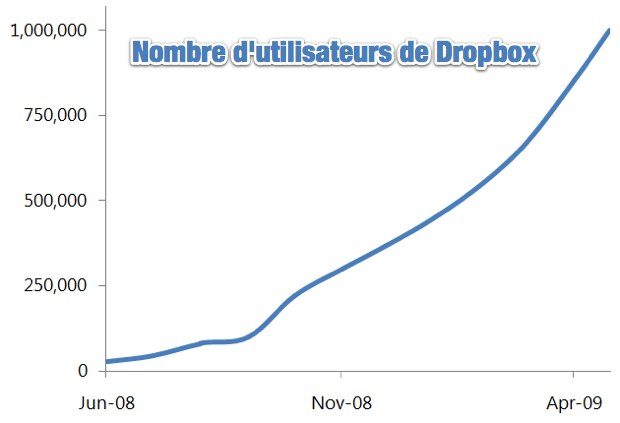
\includegraphics[height = 5cm, width = 5cm]{jpg/db8.jpg}\\
Ce graphique nous permet clairement de voir que suite à ce changement dans leur manière d'opérer au niveau marketing,
l'adoption de ce produit par les gens s'est beaucoup plus rapidement accroît.\\
Cette nouvelle méthode d'opérer en mettant les clients au centre de la publicité du produit a conduit à ce comportement type des clients :
\begin{itemize}
 \item Une personne entend parler du service DropBox par un ami, sur un blog, etc. et l'essaye.
 \item Ce nouveau client s'aperçoit que finalement DropBox assouvit un besoin non exprimé, à savoir le stockage simple de ses données.
 \item Ce même client réalise que DropBox est une solution qui marche parfaitement bien.
 \item Vu qu'il est satisfait de ce produit, cet utilisateur va vanter le service DropBox auprès de ses amis et sur des blogs.
\end{itemize}
Statistiquement, en 30 jours (Avril 2010), les utilisateurs de DropBox ont envoyé un total de 2,8 millions d'invitations à leurs amis.\\
35\% des inscriptions journalières proviennent d'invitations de clients et 20\% sont dûes au partage de fichiers ou autres.\\
Les enseignements que la startup qu'était DropBox, sont :
\begin{itemize}
 \item La capacité très importante d'adaptation rapide au marché pour répondre aux besoins des clients.
 \item Le fait que les pratiques marketing de pénétration de marché ne sont pas efficaces dans 100\% des cas.
 \item Le fait d'identifier les spécificités d'un marché et la façon dont votre produit peut être adopté pour des utilisateurs.
\end{itemize}$\\$
\textbf{Par rapport au cadre d'analyse}, nous pouvons dire que la solution DropBox suit le modèle marketing des Rendements Croissants
d'Adoption puisque :
\begin{itemize}
 \item Vu que les performances de DropBox sont améliorées lorsque beaucoup de clients font un retour sur le produit,
nous pouvons dire que DropBox applique le concept théorique d'\textbf{apprentissage par l'usage}.
 \item Concernant le fait que plus DropBox est adopté, plus son utilité augmente du fait de la taille de sa communauté,
il est possible de dire que DropBox suit le concept d'\textbf{externalité de réseau}.
 \item Cependant, l'entreprise DropBox n'est que peu concernée par les \textbf{économies d'échelle en production} du fait qu'il
s'agisse d'un produit lié à Internet, à part pour les serveurs que le service loue à l'entreprise Amazon.
 \item Plus ce service est adopté, moins il entraîne d'aversion à son encontre, malgré le fait que certaines grandes entreprises
le déconseillent (par exemple IBM) ou ont leur propre solution de stockage en ligne (Google, Apple et Microsoft).
Donc nous pouvons dire que DropBox applique le principe des \textbf{rendements croissants d'informations}.
 \item Du coté des \textbf{interrelations technologiques}, nous avons pu observer que DropBox tend à étoffer son produit en intégrant
les technologies que l'entreprise rachète donc tend à à rendre plus attractif son produit, ce qui correspond à ce principe de marketing.
 \item DropBox n'est pas en situation évidente de \textit{lock-in} face à ses concurrents puisque même si ce service cherche
à proposer le meilleur produit à ses clients, ses concurrents sont de très grosses puissances technologiques disposant de beaucoup de moyens
(Google, Apple, Microsoft notamment) et donc le marché n'est pas, pour autant, figé autour d'un seul acteur.
\end{itemize}
$\\$
\textbf{Vis à vis de ses concurrents}, DropBox a veillé à proposer non pas plusieurs produits mais à proposer du produit,
ce qui lui a permis d'accroître son image de marque et de se créer une certaine aura auprès du grand public
vu qu'elle est synonyme de qualité.
DropBox cristallise une qualité attendue de la part des utilisateurs et a un pouvoir de captation plus grand que ses concurrents
(communauté et attachement des clients).\\
Maintenant, DropBox est capable de capter une clientèle et d'être vis parmis tous les autres très gros acteurs dans ce domaine.\\
Du fait, qu'il n'y ait pas de discrimination au niveau des prix au premier abord (dans le cas où l'espace de stockage n'est pas la
priorité du client, l'inscription à DropBox est gratuite), il n'y a pas de clivage trop fort entre ceux qui possèdent un compte DropBox
et ceux qui n'en ont pas.\\
Lorsque les clients choisissent de passer à un compte premium, ils font face à une discrimination des prix du deuxième degré,
vu qu'il n'y a pas de différenciation des utilisateurs.\\
Par contre, au niveau des barrières à l'entrée pour ses concurrents, cela se joue principalement sur le coté qualité de la solution
qu'ils peuvent appporter et donc sur leurs moyens financiers du fait que DropBox est devenu dans ce domaine incontournable et incomparable
pour sa clientèle (clientèle captive).\\ \\
\textbf{Concernant la volonté de DropBox d'entrer en bourse}, nous avons pu observer qu'il s'agissait, avant tout, d'un besoin de trouver
de nouveaux investisseurs plus rapidement et plus facilement afin de lutter de manière plus efficace face à ses concurrents disposant
de lourds moyens de financement.\\
Cependant, du fait qu'il s'agisse d'une entreprise complètement axé sur Internet et sur les particuliers, comme Facebook,
entraîne une certaine méfiance de la part des marchés boursiers.
Nous avions pu observer à l'entrée en bourse de l'entreprise Facebook, la chute du cours de son action du à la méfiance générale de ce type
de produit.
Facebook ne suivait pas de modèle économique défini mais comptait avant tout sur le poids du nombre de ses utilisateurs pour
trouver des financements.\\
Pour palier ce point et donc pour rassurer les marchés, DropBox a décidé de se tourner vers un nouveau marché, en plus des particuliers,
le marché des entreprises en proposant récemment une solution de stockage adaptée aux besoins des entreprises (avec une aide au téléphone,
un service d'historique plus avancé, une sécurité accrue) afin d'attirer notamment les entreprises de développement logiciel qui souhaitent
intégrer les outils de \textit{cloud computing} pour accroître leur productivité dans le développement en parallèle
des fonctionnalités d'un produit.\\ \\
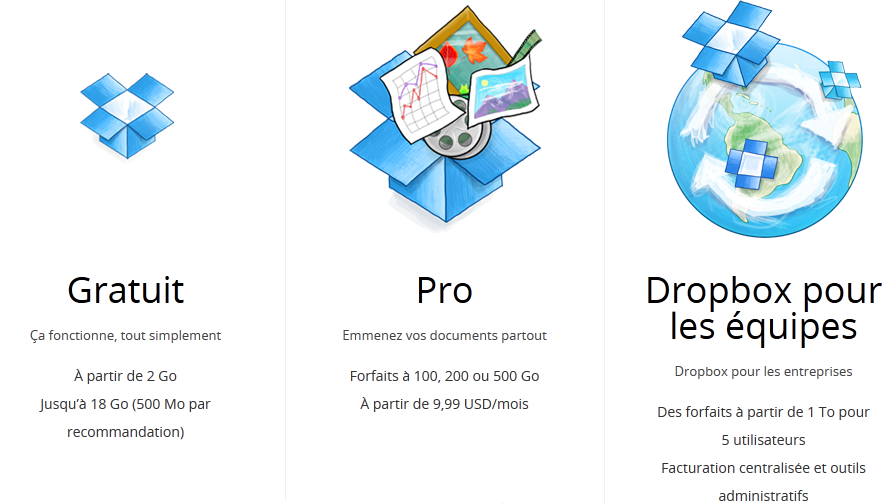
\includegraphics[height = 3.5cm, width = 5cm]{jpg/db5.png}\\
À travers cette nouveau type de comptes, DropBox cherche à se rapprocher de l'un de ces principaux concurrents, à savoir Box,
qui lui est centré sur la proposition d'une solution de \textit{cloud} aux entreprises et qui compte effectuer son entrée en bourse
au début de l'année 2014.\\ \\ \\
Pour résumer,\\ \\
\begin{tabular}{|c|c|c|}
\hline
externalités de réseau & apprentissage par l'usage & économies d'échelle en production\\
\hline
oui & oui & très peu voire non\\
\hline
\end{tabular}$\\ \\ \\$
\begin{tabular}{|c|c|c|}
\hline
rendements croissants d'informations & interrelations technologique & situation de lock-in\\
\hline
oui & oui & oui mais réversible\\
\hline
\end{tabular}
\newpage \noindent
Selon les dirigeants de DropBox, nous pouvons expliquer son succès avec les points suivants :\\ \\
\textbf{Le fait d'avoir un produit fonctionnel.}\\
Lorsque DropBox a été lancé, le marché était déjà saturé d'acteurs en compétition.\\
Malgré la forte diversité d'entreprise dans le \textit{cloud storage}, les fondateurs de DropBox se sont rendus compte que 
les utilisateurs de ces solutions n'étaient pas pleinement satisfaits (notamment grâce aux divers commentaires sur les forums et blogs).
Les produits concurrents ne fonctionnaient pas tout le temps et créaient parfois des fichiers erronés.\\
En réponse à ces produits, DropBox a décidé de créer une simple application de stockage de fichiers qui fonctionne.
À l'heure d'aujourd'hui, DropBox fait parti des solutions de stockage en ligne les plus simples et les plus efficaces.\\
Les clients parlent des bons produits, donc la première étape d'une stratégie de marketing avec du\\bouche-à-oreille est d'avoir
un produit qui fonctionne tout le temps.\\ \\
\textbf{La construction d'une communauté avant d'avoir un produit.}\\
Il ne faut pas croire qu'il est obligatoire d'avoir un produit complémentement finalisé pour que les gens en parlent.
Pour se construire cette communauté, DropBox a veillé à utiliser les pages de destination ("landing pages" en anglais,
correspondant à une page web vers laquelle renvoie un lien proposé dans le corps d'un email commercial ou d'un objet commercial)
et à créer une version beta du produit.\\
Cette façon de procéder a permis à DropBox de créer de l'intérêt de la part du public pour son produit en l'impliquant dans le processus
de fabrication et d'optimisation du produit final.\\ \\
\textbf{La question des bonnes pratiques.}\\
Le lancement du produit finalisé de DropBox n'est pas différents du plan de lancement des autres\\produits.
Ses créateurs ont donc utiliser la publicité dîte de paiement par clic (sur les publicités de sites web),
organisé une conférence pour présenter leur produit et fait appel aux services d'une entreprise pour gérer les relations publics.\\
Cependant, cette stratégie de lancement de leur produit n'a pas du tout fonctionné parce que le coût de l'acquisition d'un clients
était trop élevé du fait des dépenses liées aux mots clés dans les publicités.\\
Les méthodes plutôt traditionnelles de pénétration de marchés n'ont pas permis à DropBox de prendre du poids sur ce marché.
Mais, l'entreprise a réalisé que malgré cet échec dans la stratégie de lancement de leur produit,
elle prenait de plus en plus de place sur le marché.
Ce succès est surtout à mettre sur le compte du bouche-à-oreille concernant les qualités de DropBox.
Il a donc ensuite été question pour ses fondateurs de déterminer comment est-il possible d'obtenir ce phénonème de buzz autour d'un produit ?\\ \\
\textbf{La favorisation du bouche-à-oreille.}\\
Pour tirer pleinement de ce phénomène concernant leur produit, les créateurs de DropBox ont choisi de mettre en place tout un système
ayant pour but d'inciter leurs clients à recommender leur application aux autres.
En implémentant cette simple fonctionnalité, l'acquisition de nouveaux clients a été multipliée de 60\%.\\
En plus de ce système de recommendations, DropBox a effectué des changements sur leur produit afin de rendre plus facile pour les utilisateurs
de partager leurs satisfactions avec les autres.
Par exemple, ils ont implémenté une fonctionnalité de partage de dossiers, ce qui permet le partage d'un dossier de documents d'être partagé
avec plusieurs clients. Cette nouvelle fonctionnalité, de manière implicite, encouragé les utilisateurs à inviter leurs amis pour
partager l'accès à leurs dossiers.\\ \\
\textbf{La compréhension de ce qui marche.}\\
Afin de mesurer les effets de chacune de leurs stratégies de pénétration de marché, DropBox a mis l'accent sur la récupération de données
pour que leurs analyses découlent sur les bonnes stratégies de marketing à adopter et les investissements intéressants
de fonctionnalités pour étoffer le produit final.\\
Le but de cette démarche était de découvrir la façon dont les nouveaux utilisateurs découvraient leur application.

\newpage
\section*{Conclusion}
Pour conclure, nous pouvons dire que la solution de stockage de fichiers en ligne DropBox a su s'imposer comme une référence dans ce domaine
en priviliégeant avant tout la satisfaction du client et en étant réactif par rapport à ses choix marketing.\\
Cette entreprise a su passer d'une stratégie marketing classique à une stratégie plus complexe en faisant interagir ses clients avec ses
futurs clients (le parrainage et le partage de fichiers) ce qui lui a permis de sortir du lot vis à vis de ses concurrents.\\
Son succès est avant tout centré sur les utilisateurs lambda et beaucoup moins sur les entreprises, ce qu'elle cherche à corriger.\\
Cependant, nous avons pu observer que son avenir est plutôt flou quant à son entrée en bourse du fait d'un climat de méfiance existant
pour les valeurs technologique basée sur Internet.

\newpage
\section*{Bibliographie}
\begin{itemize}
 \item \textit{\textbf{Les modèles de compétition technologique, une revue de la littérature}},\\
de \textbf{Dominique Foray}, CNRS/ECT Lyon II, sur le site \textit{http://www.persee.fr}.
 \item \textit{\textbf{Customer Developpement Case Study : DropBox}},\\
par \textbf{Drew Houston}, sur le site \textit{http://www.justin.tv/startuplessonslearned/b/262672510}.
 \item \textit{\textbf{DropBox, Startup Lessons Learned}},\\
par \textbf{Drew Houston}, sur le site \textit{http://techcrunch.com/2011/10/19/dropbox-minimal-viable-product/}.
 \item \textit{\textbf{Marketing lessons from DropBox: A Q\&A with CEO Drew Houston}},\\
sur le site \textit{http://answers.oreilly.com/topic/1372-marketing-lessons-from-dropbox-a-qa-with-ceo-drew-houston/}
 \item \textit{\textbf{Définition des landing pages}},\\
sur le site \textit{http://www.definitions-webmarketing.com/Definition-Landing-page}
\end{itemize}

\end{document}
